% SEPTAGRAPH — NIME draft v0.1
% Compile: any modern LaTeX (Overleaf works; no local toolchain needed).
% NOTE: written on plain two-column `article` so it compiles anywhere;
% swap the preamble for the official NIME template class before submission —
% section/figure content ports unchanged.

\documentclass[10pt,twocolumn]{article}
\usepackage[margin=2cm]{geometry}
\usepackage{tikz}
\usetikzlibrary{arrows.meta,positioning,calc,decorations.pathmorphing}
\usepackage{pgfplots}
\pgfplotsset{compat=1.17}
\usepackage{booktabs}
\usepackage{amsmath}
\usepackage[hidelinks]{hyperref}

\title{\textbf{Septagraph: A Perceptual Coordinate Protocol for Live
Interaction with Interchangeable Sound Engines}}
\author{Emory Smith \\ \small maintainer@example.invalid
  \and Colton [SURNAME] \\ \small [email]}
\date{}

\begin{document}
\maketitle

% --- OLD ABSTRACT (superseded 2026-09-03; promised a neural-renderer
%     demo and a completed listening experiment before either existed;
%     kept for reference only) -----------------------------------------
% We present Septagraph, a communication protocol in which controllers and
% sound renderers share only a perceptual coordinate space: seven axes
% grounded in auditory modulation representations. A fast plane carries raw
% performance events at sub-10\,ms latency; a slow plane carries
% \emph{septagraphs} --- trajectories of distributions $\mu(t), \sigma(t)$
% over the space --- exchanged at detected gesture boundaries, so model
% latency is structurally inaudible. The controller's model never perceives
% audio: it predicts the performer, and its prediction uncertainty becomes
% the renderer's explicit, performable freedom. Captured real-world sounds
% become septagraph objects that can be geometrically mutated and
% re-rendered by any engine speaking the protocol. We demonstrate Septagraph
% with physical and digital grid controllers driving interchangeable
% renderers --- deterministic DSP, neural synthesis, and a robotic
% instrument ensemble rendered from a measured catalog --- and report on its
% use in live performance.

\begin{abstract}
We present Septagraph, a communication protocol in which controllers and
sound renderers share only a perceptual coordinate space: seven axes
grounded in auditory modulation representations, exchanged as an OSC
sublanguage on a fast plane (sub-10\,ms discrete events) and a slow plane
(\emph{septagraphs} --- trajectories of distributions $\mu(t), \sigma(t)$
over the space --- exchanged only at detected gesture boundaries, so
model latency is structurally inaudible). We ship a zero-install
browser controller/renderer pair on WebChucK that a reader can run
without downloading anything; a Machine Lab renderer that speaks the
protocol into a seven-robot ensemble from a manifest built on a measured
catalog of each robot's reachable positions; and the neuralGrid, a
physical grid, ribbon, and lidar controller. We report a latency
evaluation of the fast plane and a listening experiment testing whether
the seven axes are independently steerable and whether the same
coordinate stream is recognizable across renderers. A neural renderer
conditioned on the same axes is in progress with collaborators and is
discussed as future work.
\end{abstract}

%--------------------------------------------------------------------
\section{Introduction}
% SKELETON — emgor writes prose. Beats:
% 1. The dilemma: ML-in-the-loop instruments promise adaptivity but
%    poison directness with latency.
% 2. MIDI's lesson: radical underspecification, not rich description,
%    is what makes a control standard universal. MIDI said which note,
%    how hard, when — the instrument owned the sound.
% 3. The gap: generative audio engines have no standard control
%    vocabulary — text prompts and model-specific latents are not
%    portable. Perceptual axes are.
% 4. Thesis: we separate WHO PREDICTS THE HUMAN from WHO RENDERS THE
%    SOUND; the sides meet only in a shared perceptual space —
%    where, how tightly, when.
% 5. Forecast the demos (controller/renderer interchangeability matrix).
% intro.tex — Introduction body, \input from septagraph.tex.
% Draft for emgor to re-voice. Beats, in order:
%   1 the concrete problem (one grid, seven robots)
%   2 why note/channel vocabularies fail
%   3 MIDI's actual lesson (underspecification)
%   4 the generative-audio control gap
%   5 thesis (separation; where / how tightly / when)
%   6 contributions + the interchangeability matrix
% ACTION(emgor): confirm authorship/acknowledgment with Kapur and Colton
%   before submission (the Machine Lab is named here and in Sec. origin).

% --- 1. The problem -------------------------------------------------
The Machine Lab at CalArts is a room of seven robotic instruments ---
BreakBot, GanaPati, Tammy, Marimba, Trimpbeat, Modulettes, and
RattleTron --- some tonal, some purely percussive, each bolted to its
own spot in the room. Composers drive them today as the ensemble has
always been driven: every instrument is a separate endpoint, reached
by its own OSC address behind a MIDI channel and note number that
select a beater and a velocity. Each machine has mechanical limits the
sender must already know --- a maximum re-strike rate, a force range,
and, on GanaPati, a thermal cutout: driven too fast it overheats and
shuts down, so faster play must arrive at lower velocity or not at
all. Nothing in the message vocabulary carries any of this.

We wanted to play the room as \emph{one} instrument from one $8\times8$
grid: move a hand across it and have the sound move from drum to
marimba, dry to noisy, left to right in the room, without ever
deciding which robot to address.

% --- 2. Why notes and channels fail ---------------------------------
Note and channel vocabularies cannot express that request. In MIDI, a
robot is a channel and a beater is a note number; ``a bit noisier and
a little further left'' is not a message that exists. There is no
continuum between a drum and a marimba because there is no axis along
which they differ --- they are two channels. The same wall stands
between two software synthesizers, or between a synthesizer and a
robot: as long as the shared language names \emph{sources}, a
controller can only choose one.

% --- 3. MIDI's actual lesson ----------------------------------------
It is tempting to conclude the fix is a richer description of sound.
MIDI's history argues the opposite. MIDI became universal because it
said almost nothing --- which key, how hard, when --- and left the
instrument to own everything else. That underspecification is why a
1983 keyboard still drives a 2026 synthesizer. A control standard
survives by naming the smallest thing both sides can agree on. MIDI's
problem is not that it is thin; it is that the thin thing it names ---
a key on a keyboard --- stopped being the right primitive once the
receiver was no longer a keyboard instrument.

% --- 4. The generative-audio control gap ----------------------------
The gap is now acute. Neural and generative sound engines have no
control vocabulary beyond whatever each model happens to expose: a
text prompt, or a latent vector meaningless to any other model.
Neither is portable; neither is something a hand can play in real
time. What \emph{is} portable, across a neural engine, a deterministic
synthesizer, and a solenoid-struck drum, is a perceptual description
of the result --- how bright, how noisy, how fast it flutters, where
in the room it sits. These are the quantities a listener hears and a
performer aims for, and any engine can be asked to reach a point on
them in its own way.

% --- 5. Thesis ------------------------------------------------------
Septagraph is built on one separation: the side that \emph{predicts
the human} is kept apart from the side that \emph{renders the sound},
meeting only in a shared perceptual coordinate space expressed as an
OSC sublanguage. A controller says \emph{where} in that space a sound
should land, \emph{how tightly} ($\sigma$, the renderer's declared
freedom to deviate), and \emph{when} --- discrete events on a fast
plane no model ever touches, and slower reconfiguration delivered only
at gesture boundaries, so whatever intelligence sits behind the
controller can be arbitrarily slow without its latency ever being
heard. A renderer announces what it can reach: a continuous region for
a synthesizer, or a measured \emph{catalog} of discrete positions for a
physical ensemble, each carrying the mechanical constraints the robots
forced us to model. Neither side knows anything else about the other.

% --- 6. Contributions and the matrix --------------------------------
This paper contributes: (i) the coordinate space and its wire grammar
(Secs.~\ref{sec:space}--\ref{sec:window}); (ii) a zero-install browser
controller/renderer pair on WebChucK a reader can run without
downloading anything; (iii) a Machine Lab renderer that speaks the
protocol into the ensemble's existing OSC server from a catalog of
measured robot positions; (iv) the neuralGrid, a physical grid, ribbon,
and lidar controller; (v) a latency evaluation of the fast plane; and
(vi) a listening experiment testing whether the axes are independently
steerable and whether the same coordinate stream is recognizable across
renderers. The central evidence is an interchangeability matrix ---
controllers against renderers, every cell the same protocol stream and
a working performance (Sec.~\ref{sec:eval}). A neural renderer
conditioned on the same axes is in progress with collaborators and is
discussed as future work. Before the technical sections, we describe
where this came from, because the robots shaped most of what follows.


%--------------------------------------------------------------------
\section{Origin: Playing a Robot Orchestra as One Instrument}
\label{sec:origin}
% origin.tex — "Origin: Playing a Robot Orchestra as One Instrument",
% \input from septagraph.tex. ~half a page. Honest narrative: grid for
% robots -> what did not work -> the protocol. Draft for emgor to re-voice.
% ACTION(emgor): confirm authorship/acknowledgment with Kapur and Colton
%   before submission (the ensemble, its server lineage and its current
%   maintainer are described here; no individuals are named as authors).

Septagraph did not start as a protocol. It started as a grid.

The neuralGrid was designed in mid-2026 as a Monome-style controller
with a second job: a small local model would watch how the player
played and rewrite the grid's own layout, every change quantized to a
shared clock so the model's latency would land on a downbeat and never
be felt. Its first target was the Machine Lab. The ensemble is driven
from a Mac mini running a ChucK server whose lineage runs through
several generations of the lab's students and faculty; composers send
OSC to one port, one address per robot, and the server turns each
message into MIDI or serial commands for that machine. The obvious
first build was a direct script: grid cells hand-mapped to robots, a
pad press becoming an OSC message to the lab server. That script still
exists and is still the gig tool; it is also the end-to-end proof that
the hardware works.

Several things about the first design did not survive contact with the
room. The four ribbon sensors on the grid's edges were originally
menus --- touch one to select a mode, then scroll it --- and the
player's last-touched ribbon decided what the grid meant. In practice a
menu on a performance surface meant looking at the instrument instead
of playing it, and ``touched last'' turned sensor noise into mode
changes. The ribbons were demoted to pure modulators, one axis each,
and menus moved to a web page. Beat-quantized reconfiguration went the
same way: the robots share no clock, and the compositions written for
them assume none, so reconfiguring on a beat meant importing a
metronome nobody in the room was listening to. Reconfiguration now
lands at detected gesture boundaries --- moments of stillness in the
input stream --- which need no clock and are, in practice, the moments
when a change of mapping is least disruptive.

The robots also forced the shape of the renderer manifest. A
synthesizer can be told to reach any point in a continuous region; a
robot cannot. Each beater on each machine is one fixed sound at one
fixed place in the room, so the ensemble's reachable set is a finite
catalog of measured positions, not a bound. A catalog of positions is
still not enough: a composer who sends the same beater too many hits
per second gets softer strikes and, on GanaPati, a thermal shutdown.
So every catalog point carries its mechanical constraints --- maximum
re-strike rate and a force range --- and a controller that respects
them will never ask a robot for a roll it cannot play. This is the
part of the protocol we would not have designed for synthesizers
alone, and it is what makes a physical instrument a first-class
renderer rather than a special case.

Once the grid's output had become ``a position in a perceptual space,
with a tolerance'' rather than ``robot $n$, beater $m$'', the
separation described in the introduction was already in place: the
same stream that drives the robots drives a browser synthesizer, and
the instrument on the table no longer knows or cares which one is
listening. The rest of this paper describes that stream.


%--------------------------------------------------------------------
\section{The Space}
\label{sec:space}

Septagraph's coordinate system comprises seven axes grounded in
spectro-temporal modulation representations of auditory
perception~\cite{shamma,mcdermott}: \textbf{frequency},
\textbf{loudness}, \textbf{harmonicity} (tone--noise continuum),
\textbf{rate} (temporal modulation), \textbf{scale} (spectral
modulation), \textbf{space} (azimuth, spread, distance), and
\textbf{time}, the trajectory parameter along which the other six
evolve. The claim made for these axes is \emph{independent
steerability} --- each can be varied audibly while the others hold ---
not mathematical orthogonality. The axis set is schema-versioned;
additions bump the version, and captured material remains valid under
version tags.

A sound is not a point in this space. A sound is a
\emph{septagraph}: a trajectory of distributions $\mu(t), \sigma(t)$
over axes 1--6 along normalized time, with a single duration
parameter, so captured shapes stretch at render time
(Fig.~\ref{fig:septagraph}).

\begin{figure}[t]
\centering
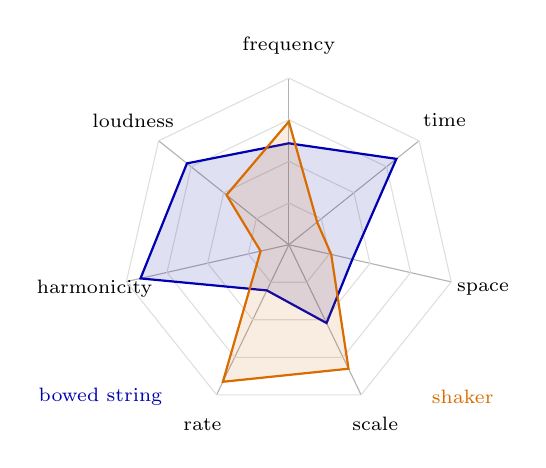
\begin{tikzpicture}[scale=0.92]
  % 7-axis radar: two example sounds
  \foreach \a/\l in {90/frequency, 141.4/loudness, 192.8/harmonicity,
                     244.3/rate, 295.7/scale, 347.1/space, 38.6/time}{
    \draw[gray!60] (0,0) -- (\a:2.3);
    \node[font=\scriptsize] at (\a:2.75) {\l};
  }
  \foreach \r in {0.575,1.15,1.725,2.3}
    \draw[gray!25] (90:\r) \foreach \a in {141.4,192.8,244.3,295.7,347.1,38.6,90}{ -- (\a:\r)};
  % Sound A: bowed string (harmonic, mid-bright, slow)
  \draw[thick,blue!70!black,fill=blue!60!black,fill opacity=0.12]
    (90:1.4) -- (141.4:1.8) -- (192.8:2.1) -- (244.3:0.7)
    -- (295.7:1.2) -- (347.1:0.9) -- (38.6:1.9) -- cycle;
  % Sound B: shaker (noisy, fast, dry)
  \draw[thick,orange!85!black,fill=orange!80!black,fill opacity=0.12]
    (90:1.7) -- (141.4:1.1) -- (192.8:0.4) -- (244.3:2.1)
    -- (295.7:1.9) -- (347.1:0.6) -- (38.6:0.5) -- cycle;
  \node[font=\scriptsize,blue!70!black]  at (-2.6,-2.1) {bowed string};
  \node[font=\scriptsize,orange!85!black] at (2.4,-2.1) {shaker};
\end{tikzpicture}
\caption{The seven Septagraph axes. Two sounds shown as single points
for illustration; in the protocol a sound is a trajectory of
distributions over the axes (Fig.~\ref{fig:septagraph}).}
\label{fig:axes}
\end{figure}

\begin{figure}[t]
\centering
\begin{tikzpicture}
\begin{axis}[width=0.98\linewidth,height=4.4cm,
  xlabel={normalized time $t$},ylabel={axis value},
  xmin=0,xmax=1,ymin=0,ymax=1,
  label style={font=\scriptsize},tick label style={font=\tiny},
  legend style={font=\tiny,draw=none,fill=none,at={(0.98,0.95)},anchor=north east}]
  % sigma band around mu (brightness-like axis of one note)
  \addplot[name path=hi,draw=none,domain=0:1,samples=60]
    {0.35+0.45*exp(-14*(x-0.12)^2)+0.18*exp(-6*(x-0.6)^2)+0.10};
  \addplot[name path=lo,draw=none,domain=0:1,samples=60]
    {0.35+0.45*exp(-14*(x-0.12)^2)+0.18*exp(-6*(x-0.6)^2)-0.10};
  \addplot[blue!30] fill between[of=hi and lo];
  \addplot[thick,blue!70!black,domain=0:1,samples=60]
    {0.35+0.45*exp(-14*(x-0.12)^2)+0.18*exp(-6*(x-0.6)^2)};
  \legend{,,$\mu(t)\pm\sigma(t)$,$\mu(t)$}
\end{axis}
\end{tikzpicture}
\caption{A septagraph, shown on one axis: the mean trajectory
$\mu(t)$ with spread $\sigma(t)$. Spread is the renderer's explicit
liberty --- underspecification made performable.}
\label{fig:septagraph}
\end{figure}

%--------------------------------------------------------------------
\section{The Protocol}
\label{sec:protocol}

Septagraph defines four broadcast message types on three planes
(Fig.~\ref{fig:arch}):

\begin{itemize}
\item \texttt{/manifest} (session plane): a renderer joining the
session declares its reachable region --- a continuous bound for
synthesis engines, or a \emph{measured catalog} for physical
instruments, each catalog point carrying instrument identity, room
position, and mechanical constraints (maximum re-strike rate, force
range). This is the only renderer-to-controller channel; manifests
may be re-announced when capability changes. Controllers mirror this
with an \emph{input manifest} declaring each device's channels by
geometry (1D/2D/3D, discrete/continuous, display capability), making
the controller brain device-agnostic.
\item \texttt{/shape} (slow plane): septagraphs and window
configurations, applied only at \emph{detected gesture boundaries} ---
moments of stillness in the interaction stream. The mapping never
changes mid-gesture; a model authoring shapes may therefore be
arbitrarily slow without its latency ever being audible. No global
clock is assumed.
\item \texttt{/hit} (fast plane): onset/release events with voice
identity, velocity, and window-local coordinates, delivered sub-10\,ms
with no model in the path.
\item \texttt{/move} (fast plane): continuous channel streams
(ribbon, pressure, height) at 50--100\,Hz, voice-bound when
modulating a held note.
\end{itemize}

\begin{figure}[t]
\centering
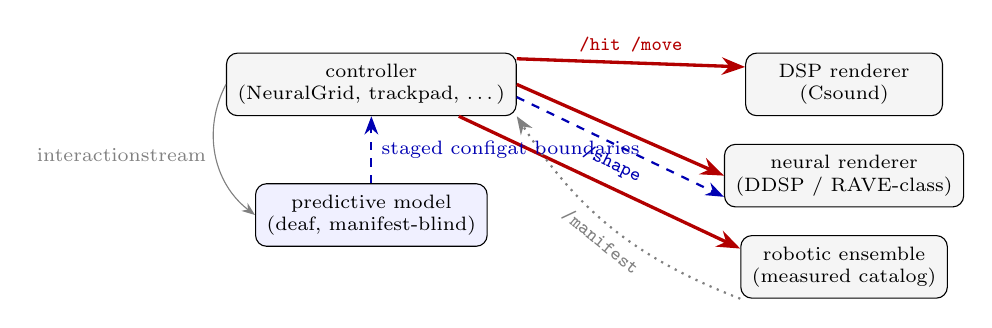
\begin{tikzpicture}[font=\scriptsize,
  box/.style={draw,rounded corners,align=center,inner sep=4pt},
  fast/.style={-{Stealth},very thick,red!70!black},
  slow/.style={-{Stealth},thick,blue!70!black,dashed},
  sess/.style={-{Stealth},thick,gray,dotted}]
  \node[box,fill=gray!8,minimum width=2.6cm] (ctl) {controller\\(NeuralGrid, trackpad, \dots)};
  \node[box,fill=gray!8,right=2.9cm of ctl,minimum width=2.5cm] (r1) {DSP renderer\\(Csound)};
  \node[box,fill=gray!8,below=0.35cm of r1] (r2) {neural renderer\\(DDSP / RAVE-class)};
  \node[box,fill=gray!8,below=0.35cm of r2] (r3) {robotic ensemble\\(measured catalog)};
  \node[box,fill=blue!6,below=0.85cm of ctl,minimum width=2.6cm] (model)
    {predictive model\\(deaf, manifest-blind)};
  \draw[fast] (ctl.10) -- node[above]{\texttt{/hit /move}} (r1.170);
  \draw[fast] (ctl.east) -- (r2.west);
  \draw[fast] (ctl.-20) -- (r3.170);
  \draw[slow] (ctl.-5) -- node[below,sloped]{\texttt{/shape}} (r2.190);
  \draw[sess] (r3.south west) to[bend left=18]
    node[below,sloped]{\texttt{/manifest}} (ctl.south east);
  \draw[slow] (model) -- node[right]{staged config\\at boundaries} (ctl);
  \draw[-{Stealth},gray] (ctl.west) to[bend right=40]
    node[left]{interaction\\stream} (model.west);
\end{tikzpicture}
\caption{Architecture. Fast plane (solid red) is never touched by a
model; the slow plane (dashed) lands only at gesture boundaries;
the session plane (dotted) carries capability manifests --- the only
renderer-to-controller channel.}
\label{fig:arch}
\end{figure}

%--------------------------------------------------------------------
\section{The Window}
\label{sec:window}

The controller's model never maps gestures to coordinates. A
deterministic, axis-aligned \emph{window} --- center and extent per
axis plus a discrete assignment map from device axes to space axes ---
projects device space into the coordinate space instantly
(Fig.~\ref{fig:window}). The model's sole authority is to move,
resize, and reassign the window \emph{between} gestures. Extent (the
playable range) and spread ($\sigma$, the renderer's liberty) are
distinct quantities: the first is deterministic configuration, the
second is model uncertainty.

Renderer manifests are merged into a density field over the space;
window cells snap to measured catalog points first, with continuous
renderers filling the intervals. A configuration holds two windows:
a \emph{play} layer and a \emph{loop} layer, the latter frozen by
default so replayed material keeps its sound while the play window
travels.

\begin{figure}[t]
\centering
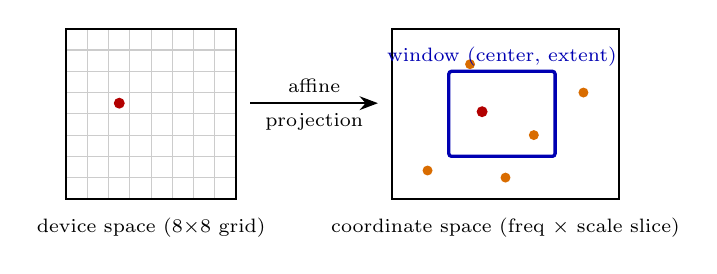
\begin{tikzpicture}[font=\scriptsize,scale=0.9]
  % device grid
  \draw[step=0.3,gray!40] (0,0) grid (2.4,2.4);
  \draw[thick] (0,0) rectangle (2.4,2.4);
  \node at (1.2,-0.4) {device space (8$\times$8 grid)};
  \fill[red!70!black] (0.75,1.35) circle (2.2pt);
  % space with window
  \begin{scope}[shift={(4.6,0)}]
    \draw[thick] (0,0) rectangle (3.2,2.4);
    \node at (1.6,-0.4) {coordinate space (freq $\times$ scale slice)};
    % catalog points
    \foreach \p in {(0.5,0.4),(1.1,1.9),(2.0,0.9),(2.7,1.5),(1.6,0.3)}
      \fill[orange!85!black] \p circle (2pt);
    % window
    \draw[very thick,blue!70!black,rounded corners=1pt] (0.8,0.6) rectangle (2.3,1.8);
    \node[blue!70!black] at (1.55,2.0) {window (center, extent)};
    \fill[red!70!black] (1.27,1.23) circle (2.2pt);
  \end{scope}
  \draw[-{Stealth},thick] (2.6,1.35) -- node[above]{affine} node[below]{projection} (4.4,1.35);
\end{tikzpicture}
\caption{Window projection: a pad press maps deterministically
through the current window. Orange points are a physical ensemble's
measured catalog; window cells snap to them first. The model only
moves the window, and only between gestures.}
\label{fig:window}
\end{figure}

%--------------------------------------------------------------------
\section{Uncertainty as Vocabulary}
% SKELETON: sigma sourced from mixture entropy of the predictive
% model; tight = faithful rendering, wide = renderer roams; for the
% robotic ensemble, wide sigma = freedom to choose among nearby
% physical notes (orchestration freedom). Underspecification is the
% expressive material — MIDI's lesson made explicit and performable.
% uncertainty.tex — "Uncertainty as Vocabulary", \input from septagraph.tex.

Every coordinate on the wire carries a $\sigma$ alongside its $\mu$
(Sec.~\ref{sec:space}), and $\sigma$ is not measurement noise to be
minimized: it is the renderer's declared liberty to deviate from the
requested point, and a controller sets it on purpose. In v1, $\sigma$
is authored --- fixed by a manifest point's measurement uncertainty, or
set explicitly by a controller preset; a future controller model could
instead derive it from the entropy of its own predictive mixture over
where the player is heading, wide when unsure, narrow when confident,
but that derivation is design, not something this paper builds or
measures.

What $\sigma$ licenses depends on the renderer. A continuous synthesis
engine draws once per hit from within $\mu \pm \sigma$ on each axis ---
the reference ChucK renderer samples a single point per onset rather
than wandering continuously mid-note, so a wide $\sigma$ is heard as
hit-to-hit variation, not vibrato. A catalog renderer instead treats
$\sigma$ as \emph{orchestration freedom}: given $\sigma > 0$ it may
realize the hit at any catalog point within $\sigma$ per axis rather
than the nearest one, and with $\sigma = 0$ it always picks nearest ---
this is implemented, not proposed (\texttt{within\_sigma} selection over
the measured catalog). Concretely, $\sigma = 1$ on an axis tells a
renderer ``your choice on this axis,'' the same abdication a
controller makes implicitly whenever MIDI leaves an instrument's timbre
unspecified; Septagraph just gives that abdication a number instead of
leaving it silent.

$\sigma$ (spread) is not extent (Sec.~\ref{sec:window}): extent is the
controller's playable range and never leaves the controller, while
$\sigma$ travels with the coordinate and is the renderer's business.
The two combine, not compete, when a shape rides a hit: a knot's own
spread and the triggering hit's spread add in quadrature,
\begin{equation}
\sigma_{\mathrm{eff}} = \sqrt{\sigma_{\mathrm{hit}}^2 + \sigma_{\mathrm{knot}}^2},
\end{equation}
so a precise hit under a loose shape, or a loose hit under a precise
shape, both still yield one well-defined liberty at render time.


%--------------------------------------------------------------------
\section{The Deaf Controller}
% SKELETON: one tiny causal sequence model (~10^5–10^6 params, MDN
% head) trained self-supervised on next-action prediction + behavior
% cloning of the player's manual configuration choices. It never
% hears audio and never reads manifests: it understands only the
% human's habits in the space. Cold start: system fully usable with
% the model absent (manual -> log -> train -> enable). Looping is a
% deterministic live-layer function; loop "effects" are geometric
% transforms on septagraphs (stutter = chopped time axis, smear =
% widened sigma).
% deaf_controller.tex — "The Deaf Controller", \input from septagraph.tex.

The architecture commits to a separation stronger than convenience: the
controller side never hears audio, and the renderer side never sees
the player. Neither side models the other directly; they meet only in
the shared coordinate space, through messages that carry a position
and a liberty and nothing about who sent them or why. This is what
keeps a synthesis engine, a physical instrument, and eventually a
predictive model interchangeable on either side of the protocol ---
none of them needs to know what the others are.

The window (Sec.~\ref{sec:window}) is the only mapping mechanism
between a gesture and a coordinate, and it is deterministic and
inspectable: center, extent, and an assignment table, applied by fixed
arithmetic with no model in the loop. Any intelligence placed on the
controller side is restricted to one authority --- moving, resizing,
and reassigning the window \emph{between} gestures, on the slow plane
--- and is categorically forbidden from touching \texttt{/hit} or
\texttt{/move}: those two message types are emitted by the window
projection alone, every time, regardless of what does or does not sit
behind it.

That restriction is also a cold-start law: the system is fully usable
with no model present, because a model was never load-bearing for
basic operation, only for automating window placement a player would
otherwise do by hand. Every demo in this paper --- every renderer,
every controller geometry, the latency measurement in
Sec.~\ref{sec:eval} --- runs exactly this way, model-free. The
predictive, deaf-aimed sequence model sketched for the window is future
work; this paper evaluates the protocol and the window on their own
merits and does not claim a working predictive model. That claim is
not a hedge so much as a structural guarantee: because the fast plane
is pure arithmetic with no branch for ``is a model attached,'' the
latency measurement in Sec.~\ref{sec:eval} is what model-on looks like
too --- there is no separate code path for the model to slow down.


%--------------------------------------------------------------------
\section{Shape Capture}
% SKELETON: modulation filterbank + curve fit turns recorded audio
% into septagraphs; capture -> geometric mutation -> re-render by any
% engine. The robotic catalog is built the same way: every physical
% note measured through the front-end becomes a point in the space —
% the template for mapping any acoustic instrument into the format.
% capture.tex — "Shape Capture", \input from septagraph.tex.

A recorded sound becomes a septagraph by the same route the axes were
grounded in: a modulation-filterbank analysis front end, run frame by
frame, converts a waveform into a trajectory over the six perceptual
axes~\cite{shamma,mcdermott}. We measure spectral centroid for
\texttt{freq}, RMS energy for \texttt{loud}, one minus spectral
flatness for \texttt{harm}, the dominant peak of each frame's envelope
modulation spectrum for \texttt{rate}, and the ripple density of the
log-magnitude spectrum for \texttt{scale}, mirroring the descriptor
families surveyed by the Timbre Toolbox~\cite{peeters2011}; each axis's
$\mu(t)$ is the frame-wise value and its $\sigma(t)$ is the frame-wise
standard deviation over a short analysis window, so a source that
wavers on an axis reports its own wavering rather than a false point
estimate. This front end is general: it is the same procedure by which
the Machine Lab catalog is populated, one measured strike per
manifest point, and it is offered as the template for bringing any
acoustic instrument --- not only the seven robots --- into the format.

Capture is only half the vocabulary; the other half is what a looper
does to a captured septagraph, and every operation we define is a
geometric transform on the trajectory rather than a new audio effect
per renderer. \emph{Stutter} chops the time axis, repeating a sub-span
of knots; \emph{smear} widens $\sigma(t)$ uniformly, trading definition
for renderer liberty without moving $\mu$; \emph{displace} translates
the \texttt{freq} trajectory by a constant offset; \emph{reverse} flips
the knot order in $t$. Because these act on the septagraph itself and
not on any one renderer's audio, the same stutter or smear replays
correctly whether the loop layer (Sec.~\ref{sec:window}) is driving the
DSP reference renderer, a neural voice, or the robotic ensemble ---
one looping vocabulary, defined once in coordinate space, inherited by
every engine that speaks the protocol.


%--------------------------------------------------------------------
\section{Implementations and Evaluation}
% SKELETON:
% - Controllers: NeuralGrid (8x8 grid + 4 softpots + lidar, ESP32->Pi),
%   digital controller (trackpad/web).
% - Renderers: Csound (deterministic reference), DDSP (neural
%   reference; harmonic/noise split maps directly onto harmonicity),
%   collaborator RAVE-class engine, robotic ensemble via
%   nearest-neighbor over the measured catalog; residual rendering =
%   synthesis completes the ensemble between catalog points.
% - THE MATRIX FIGURE: controllers x renderers, every cell a working
%   demo (the central evidence).
% - Latency table: hot path with model on vs off; boundary-swap
%   timing.
% - Performance reports / practice-based reflection.

\begin{table}[h]\centering\scriptsize
\begin{tabular}{lccc}
\toprule
 & Csound & DDSP/neural & robotic ensemble \\
\midrule
NeuralGrid (physical) & $\checkmark$ & $\checkmark$ & $\checkmark$ \\
digital controller    & $\checkmark$ & $\checkmark$ & $\checkmark$ \\
\bottomrule
\end{tabular}
\caption{Interchangeability matrix (target). Every cell: the same
protocol stream, a working performance.}
\end{table}

%--------------------------------------------------------------------
\section{Related Work and Limitations}
% SKELETON — own the attacks before reviewers do:
% - Adaptive mapping / IML lineage (Wekinator etc.): prior work puts
%   the model in or near the control loop; here inference may never
%   touch the hot path, and uncertainty is part of the vocabulary.
% - MIDI/MPE/OSC: notes vs perceptual position; OSC is transport,
%   not vocabulary.
% - Perceptual grounding contestable: steerability claim + versioned
%   schema, not a completed psychoacoustics.
% - Deaf-aiming: grounded by behavior cloning of manual play;
%   demonstrated, not argued.
% - Same shape -> different renderers -> different sound: feature,
%   not bug (the MIDI defense).

% related_work.tex — Task 5.1. Referenced by % related_work.tex — Task 5.1. Referenced by % related_work.tex — Task 5.1. Referenced by \input{related_work} inside
% \section{Related Work and Limitations} in septagraph.tex. Every \cite key
% here is defined in septagraph.bib; every entry was web-verified (see
% septagraph.bib header).

\subsection{Perceptual control spaces}
Wessel's timbre space~\cite{wessel1979}, built from the multidimensional
scaling of instrument tones by Grey~\cite{grey1977}, first proposed that
low-dimensional perceptual coordinates --- not instrument-specific
parameters --- should drive musical control, with later tools such as the
Timbre Toolbox~\cite{peeters2011} operationalising the descriptors those
spaces are built from. Wessel's space is Septagraph's direct ancestor.
The difference is architectural, not conceptual: Wessel's space configures
a single synthesizer, while Septagraph is a versioned, protocol-level space
shared across arbitrarily many heterogeneous renderers at once, and it
carries distributions $\mu(t),\sigma(t)$ over time rather than fixed
points, so a controller addresses a population of engines rather than
tuning one.

\subsection{Corpus-based and catalog rendering}
Schwarz's CataRT~\cite{schwarz2006catart} and the corpus-based
concatenative synthesis literature it surveys~\cite{schwarz2007corpus}
render a target position in descriptor space by nearest-neighbour lookup
into a corpus of recorded units --- the closest prior art to a Septagraph
catalog renderer, and the template for treating discrete sound sources as
points in a continuous space. Septagraph differs in where the catalog
lives and who chooses within it: a CataRT corpus is local to one engine
and queried by unit selection, whereas a Septagraph catalog is a
\emph{renderer's own capability declaration} on a shared protocol,
published to controllers that may be manifest-blind, with $\sigma$
functioning as explicit orchestration freedom that lets the renderer, not
the controller, pick among catalog points within tolerance.

\subsection{Control protocols and capability negotiation}
Open Sound Control~\cite{wrightfreed1997,wright2005} supplies transport
and addressing, not vocabulary, and SpatDIF~\cite{spatdif2013} shows the
pattern Septagraph follows: a domain-specific OSC sublanguage layered on
that transport, there for spatial scene description, here for perceptual
position. MIDI 2.0's Capability Inquiry and Property
Exchange~\cite{midici} and MPE~\cite{mpe2018} are the closest analogues to
Septagraph's \texttt{/manifest} plane and per-voice addressing
respectively: MIDI-CI lets a device declare which features and properties
it supports, and MPE gives each note its own channel for continuous
expression. Septagraph's manifest declares something categorically
different from a MIDI-CI property list: not supported messages or
parameters, but a renderer's reachable region of \emph{perceptual space}
--- a continuous bound or a measured catalog with per-point mechanical
constraints --- so a controller can aim at what a renderer can actually
sound like, not just what commands it accepts.

\subsection{Mapping and interactive machine learning}
Hunt and Wanderley's studies of performer-to-synthesis
mapping~\cite{huntwanderley2002,huntwanderleyparadis2003} established that
the mapping layer, not the interface or the sound engine alone, defines an
electronic instrument's character; Fiebrink's
Wekinator~\cite{fiebrink2009wekinator,fiebrink2011thesis} and the
interactive machine learning tradition it anchors
work~\cite{fiebrinkcaramiaux2018,caramiauxtanaka2013,francoise2014} put a
trained model directly in that mapping layer, learned from human-supplied
examples. Septagraph keeps this lineage's insight that mapping deserves
first-class design attention but relocates any model out of the
gesture-to-sound path entirely: a Septagraph model, when present, only
repositions the deterministic window between gestures, so no inference
latency can ever land inside a note.

\subsection{Robotic musicianship}
Kapur's survey of robotic musical instruments~\cite{kapur2005history} and
ensembles such as LEMUR~\cite{singer2004lemur}, the KarmetiK Machine
Orchestra~\cite{kapur2011machineorchestra}, and Weinberg and
collaborators' Haile and Shimon
platforms~\cite{weinbergdriscoll2006,hoffmanweinberg2010} demonstrate that
heterogeneous mechanical ensembles can be played expressively, generally
through instrument-specific control code or listening-based
improvisation. Septagraph's robotic renderer is architecturally the same
kind of catalog renderer as any synthesis engine on the protocol: the
same coordinate stream that drives a DSP or neural voice also drives the
Machine Lab ensemble, so a controller built with no knowledge of any
particular robot can still address it correctly.

\subsection{Generative audio renderers}
Differentiable and neural synthesis engines such as
DDSP~\cite{engel2020ddsp} and RAVE~\cite{caillonesling2021} expose
continuous, learned control spaces (pitch/loudness, or a learned latent)
that make them natural Septagraph renderers: DDSP's harmonic/noise split
in particular maps directly onto the harmonicity axis. Septagraph treats
such an engine's latent or parameter space as one more manifest to
declare bounds for, rather than requiring the space itself to be
perceptually grounded --- grounding is the controller's job, not every
renderer's.

\subsection{Limitations}
Septagraph's perceptual grounding rests on a claim of independent
steerability~\cite{shamma,mcdermott,wessel1979,grey1977}, not on a
completed psychoacoustic theory; the axis set is deliberately
versioned so it can be revised as that grounding is tested rather than
frozen prematurely. The controller's model, when present, never hears
audio and is aimed only by behaviour cloning of a performer's manual
window choices --- a deaf-aiming strategy that this paper demonstrates
rather than argues for in the abstract. That the same septagraph produces
a different sound on each renderer is a deliberate design choice, not an
oversight: MIDI's note numbers do the same across synthesizers, and
underspecification is what let it outlive any one instrument. Finally,
this paper reports a model-free system end to end; the predictive,
manifest-blind controller model sketched in Section~\ref{sec:window} is
future work, not a result claimed here.
 inside
% \section{Related Work and Limitations} in septagraph.tex. Every \cite key
% here is defined in septagraph.bib; every entry was web-verified (see
% septagraph.bib header).

\subsection{Perceptual control spaces}
Wessel's timbre space~\cite{wessel1979}, built from the multidimensional
scaling of instrument tones by Grey~\cite{grey1977}, first proposed that
low-dimensional perceptual coordinates --- not instrument-specific
parameters --- should drive musical control, with later tools such as the
Timbre Toolbox~\cite{peeters2011} operationalising the descriptors those
spaces are built from. Wessel's space is Septagraph's direct ancestor.
The difference is architectural, not conceptual: Wessel's space configures
a single synthesizer, while Septagraph is a versioned, protocol-level space
shared across arbitrarily many heterogeneous renderers at once, and it
carries distributions $\mu(t),\sigma(t)$ over time rather than fixed
points, so a controller addresses a population of engines rather than
tuning one.

\subsection{Corpus-based and catalog rendering}
Schwarz's CataRT~\cite{schwarz2006catart} and the corpus-based
concatenative synthesis literature it surveys~\cite{schwarz2007corpus}
render a target position in descriptor space by nearest-neighbour lookup
into a corpus of recorded units --- the closest prior art to a Septagraph
catalog renderer, and the template for treating discrete sound sources as
points in a continuous space. Septagraph differs in where the catalog
lives and who chooses within it: a CataRT corpus is local to one engine
and queried by unit selection, whereas a Septagraph catalog is a
\emph{renderer's own capability declaration} on a shared protocol,
published to controllers that may be manifest-blind, with $\sigma$
functioning as explicit orchestration freedom that lets the renderer, not
the controller, pick among catalog points within tolerance.

\subsection{Control protocols and capability negotiation}
Open Sound Control~\cite{wrightfreed1997,wright2005} supplies transport
and addressing, not vocabulary, and SpatDIF~\cite{spatdif2013} shows the
pattern Septagraph follows: a domain-specific OSC sublanguage layered on
that transport, there for spatial scene description, here for perceptual
position. MIDI 2.0's Capability Inquiry and Property
Exchange~\cite{midici} and MPE~\cite{mpe2018} are the closest analogues to
Septagraph's \texttt{/manifest} plane and per-voice addressing
respectively: MIDI-CI lets a device declare which features and properties
it supports, and MPE gives each note its own channel for continuous
expression. Septagraph's manifest declares something categorically
different from a MIDI-CI property list: not supported messages or
parameters, but a renderer's reachable region of \emph{perceptual space}
--- a continuous bound or a measured catalog with per-point mechanical
constraints --- so a controller can aim at what a renderer can actually
sound like, not just what commands it accepts.

\subsection{Mapping and interactive machine learning}
Hunt and Wanderley's studies of performer-to-synthesis
mapping~\cite{huntwanderley2002,huntwanderleyparadis2003} established that
the mapping layer, not the interface or the sound engine alone, defines an
electronic instrument's character; Fiebrink's
Wekinator~\cite{fiebrink2009wekinator,fiebrink2011thesis} and the
interactive machine learning tradition it anchors
work~\cite{fiebrinkcaramiaux2018,caramiauxtanaka2013,francoise2014} put a
trained model directly in that mapping layer, learned from human-supplied
examples. Septagraph keeps this lineage's insight that mapping deserves
first-class design attention but relocates any model out of the
gesture-to-sound path entirely: a Septagraph model, when present, only
repositions the deterministic window between gestures, so no inference
latency can ever land inside a note.

\subsection{Robotic musicianship}
Kapur's survey of robotic musical instruments~\cite{kapur2005history} and
ensembles such as LEMUR~\cite{singer2004lemur}, the KarmetiK Machine
Orchestra~\cite{kapur2011machineorchestra}, and Weinberg and
collaborators' Haile and Shimon
platforms~\cite{weinbergdriscoll2006,hoffmanweinberg2010} demonstrate that
heterogeneous mechanical ensembles can be played expressively, generally
through instrument-specific control code or listening-based
improvisation. Septagraph's robotic renderer is architecturally the same
kind of catalog renderer as any synthesis engine on the protocol: the
same coordinate stream that drives a DSP or neural voice also drives the
Machine Lab ensemble, so a controller built with no knowledge of any
particular robot can still address it correctly.

\subsection{Generative audio renderers}
Differentiable and neural synthesis engines such as
DDSP~\cite{engel2020ddsp} and RAVE~\cite{caillonesling2021} expose
continuous, learned control spaces (pitch/loudness, or a learned latent)
that make them natural Septagraph renderers: DDSP's harmonic/noise split
in particular maps directly onto the harmonicity axis. Septagraph treats
such an engine's latent or parameter space as one more manifest to
declare bounds for, rather than requiring the space itself to be
perceptually grounded --- grounding is the controller's job, not every
renderer's.

\subsection{Limitations}
Septagraph's perceptual grounding rests on a claim of independent
steerability~\cite{shamma,mcdermott,wessel1979,grey1977}, not on a
completed psychoacoustic theory; the axis set is deliberately
versioned so it can be revised as that grounding is tested rather than
frozen prematurely. The controller's model, when present, never hears
audio and is aimed only by behaviour cloning of a performer's manual
window choices --- a deaf-aiming strategy that this paper demonstrates
rather than argues for in the abstract. That the same septagraph produces
a different sound on each renderer is a deliberate design choice, not an
oversight: MIDI's note numbers do the same across synthesizers, and
underspecification is what let it outlive any one instrument. Finally,
this paper reports a model-free system end to end; the predictive,
manifest-blind controller model sketched in Section~\ref{sec:window} is
future work, not a result claimed here.
 inside
% \section{Related Work and Limitations} in septagraph.tex. Every \cite key
% here is defined in septagraph.bib; every entry was web-verified (see
% septagraph.bib header).

\subsection{Perceptual control spaces}
Wessel's timbre space~\cite{wessel1979}, built from the multidimensional
scaling of instrument tones by Grey~\cite{grey1977}, first proposed that
low-dimensional perceptual coordinates --- not instrument-specific
parameters --- should drive musical control, with later tools such as the
Timbre Toolbox~\cite{peeters2011} operationalising the descriptors those
spaces are built from. Wessel's space is Septagraph's direct ancestor.
The difference is architectural, not conceptual: Wessel's space configures
a single synthesizer, while Septagraph is a versioned, protocol-level space
shared across arbitrarily many heterogeneous renderers at once, and it
carries distributions $\mu(t),\sigma(t)$ over time rather than fixed
points, so a controller addresses a population of engines rather than
tuning one.

\subsection{Corpus-based and catalog rendering}
Schwarz's CataRT~\cite{schwarz2006catart} and the corpus-based
concatenative synthesis literature it surveys~\cite{schwarz2007corpus}
render a target position in descriptor space by nearest-neighbour lookup
into a corpus of recorded units --- the closest prior art to a Septagraph
catalog renderer, and the template for treating discrete sound sources as
points in a continuous space. Septagraph differs in where the catalog
lives and who chooses within it: a CataRT corpus is local to one engine
and queried by unit selection, whereas a Septagraph catalog is a
\emph{renderer's own capability declaration} on a shared protocol,
published to controllers that may be manifest-blind, with $\sigma$
functioning as explicit orchestration freedom that lets the renderer, not
the controller, pick among catalog points within tolerance.

\subsection{Control protocols and capability negotiation}
Open Sound Control~\cite{wrightfreed1997,wright2005} supplies transport
and addressing, not vocabulary, and SpatDIF~\cite{spatdif2013} shows the
pattern Septagraph follows: a domain-specific OSC sublanguage layered on
that transport, there for spatial scene description, here for perceptual
position. MIDI 2.0's Capability Inquiry and Property
Exchange~\cite{midici} and MPE~\cite{mpe2018} are the closest analogues to
Septagraph's \texttt{/manifest} plane and per-voice addressing
respectively: MIDI-CI lets a device declare which features and properties
it supports, and MPE gives each note its own channel for continuous
expression. Septagraph's manifest declares something categorically
different from a MIDI-CI property list: not supported messages or
parameters, but a renderer's reachable region of \emph{perceptual space}
--- a continuous bound or a measured catalog with per-point mechanical
constraints --- so a controller can aim at what a renderer can actually
sound like, not just what commands it accepts.

\subsection{Mapping and interactive machine learning}
Hunt and Wanderley's studies of performer-to-synthesis
mapping~\cite{huntwanderley2002,huntwanderleyparadis2003} established that
the mapping layer, not the interface or the sound engine alone, defines an
electronic instrument's character; Fiebrink's
Wekinator~\cite{fiebrink2009wekinator,fiebrink2011thesis} and the
interactive machine learning tradition it anchors
work~\cite{fiebrinkcaramiaux2018,caramiauxtanaka2013,francoise2014} put a
trained model directly in that mapping layer, learned from human-supplied
examples. Septagraph keeps this lineage's insight that mapping deserves
first-class design attention but relocates any model out of the
gesture-to-sound path entirely: a Septagraph model, when present, only
repositions the deterministic window between gestures, so no inference
latency can ever land inside a note.

\subsection{Robotic musicianship}
Kapur's survey of robotic musical instruments~\cite{kapur2005history} and
ensembles such as LEMUR~\cite{singer2004lemur}, the KarmetiK Machine
Orchestra~\cite{kapur2011machineorchestra}, and Weinberg and
collaborators' Haile and Shimon
platforms~\cite{weinbergdriscoll2006,hoffmanweinberg2010} demonstrate that
heterogeneous mechanical ensembles can be played expressively, generally
through instrument-specific control code or listening-based
improvisation. Septagraph's robotic renderer is architecturally the same
kind of catalog renderer as any synthesis engine on the protocol: the
same coordinate stream that drives a DSP or neural voice also drives the
Machine Lab ensemble, so a controller built with no knowledge of any
particular robot can still address it correctly.

\subsection{Generative audio renderers}
Differentiable and neural synthesis engines such as
DDSP~\cite{engel2020ddsp} and RAVE~\cite{caillonesling2021} expose
continuous, learned control spaces (pitch/loudness, or a learned latent)
that make them natural Septagraph renderers: DDSP's harmonic/noise split
in particular maps directly onto the harmonicity axis. Septagraph treats
such an engine's latent or parameter space as one more manifest to
declare bounds for, rather than requiring the space itself to be
perceptually grounded --- grounding is the controller's job, not every
renderer's.

\subsection{Limitations}
Septagraph's perceptual grounding rests on a claim of independent
steerability~\cite{shamma,mcdermott,wessel1979,grey1977}, not on a
completed psychoacoustic theory; the axis set is deliberately
versioned so it can be revised as that grounding is tested rather than
frozen prematurely. The controller's model, when present, never hears
audio and is aimed only by behaviour cloning of a performer's manual
window choices --- a deaf-aiming strategy that this paper demonstrates
rather than argues for in the abstract. That the same septagraph produces
a different sound on each renderer is a deliberate design choice, not an
oversight: MIDI's note numbers do the same across synthesizers, and
underspecification is what let it outlive any one instrument. Finally,
this paper reports a model-free system end to end; the predictive,
manifest-blind controller model sketched in Section~\ref{sec:window} is
future work, not a result claimed here.


%--------------------------------------------------------------------
\section{Conclusion}
% SKELETON (emgor writes): one law restated — the model never touches
% the hot path; it moves the instrument through sound space between
% gestures. Sigma as the expressive material of the generative-audio
% era. Future: more renderers, septagraph libraries from captured
% sound, the space as a versioned standard. Close on the room-scale
% vision: any controller, any engine, one coordinate system.

% Superseded by septagraph.bib (Task 5.1) — kept commented, not deleted.
% \begin{thebibliography}{9}\scriptsize
% \bibitem{shamma} T. Chi, P. Ru, S. Shamma. Multiresolution
% spectrotemporal analysis of complex sounds. \emph{JASA}, 2005.
% \bibitem{mcdermott} J. McDermott, E. Simoncelli. Sound texture
% perception via statistics of the auditory periphery. \emph{Neuron}, 2011.
% % TODO: Fiebrink (Wekinator), Hunt & Wanderley (mapping), MIDI/MPE,
% % OSC (Wright), DDSP (Engel et al.), RAVE (Caillon & Esling),
% % NIME adaptive-interface lineage.
% \end{thebibliography}

\bibliographystyle{plain}
\bibliography{septagraph}

\end{document}
